\documentclass[]{beamer}
\usepackage{amssymb,amsmath}
\usepackage{fixltx2e}
\usepackage{lmodern}
\usepackage{tikz}
\IfFileExists{upquote.sty}{\usepackage{upquote}}{}
\IfFileExists{microtype.sty}{\usepackage{microtype}}{}

\usetheme{Warsaw}
\usecolortheme{crane}
\usebackgroundtemplate{%
\tikz\node[opacity=0.2] {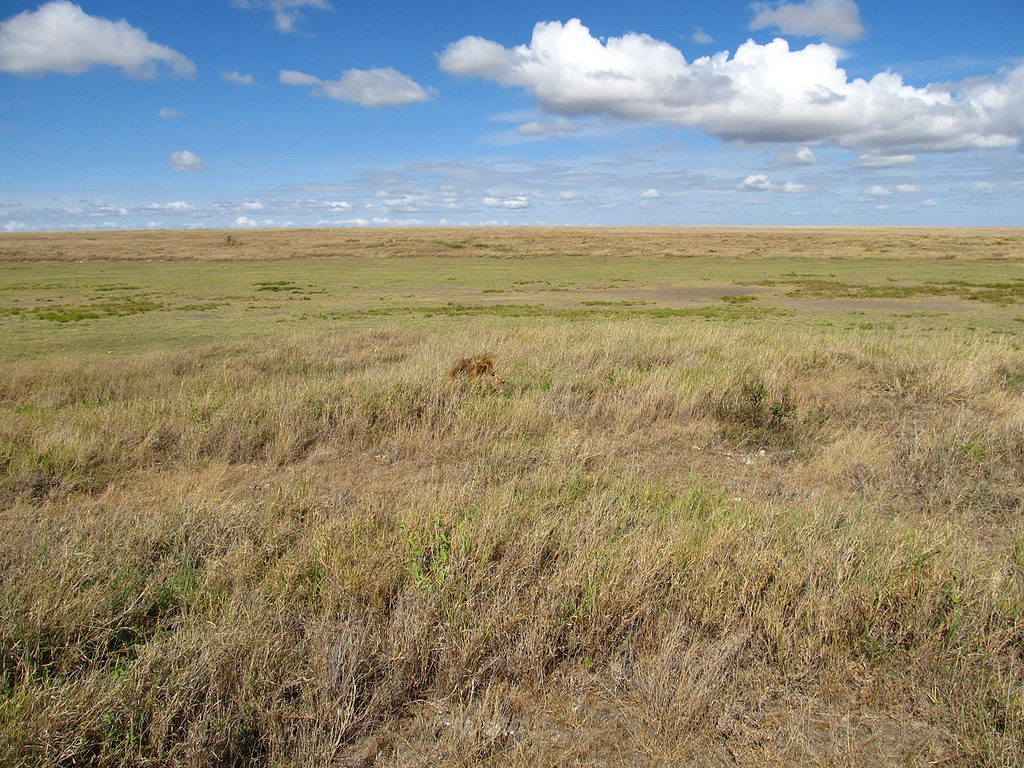
\includegraphics[height=\paperheight,width=\paperwidth]{images/Serengeti_background.jpg}};}

\setbeamercolor{mycolor}{fg=red,bg=olive}

\defbeamertemplate*{footline}{shadow theme}{%
\leavevmode%
\hbox{\begin{beamercolorbox}[wd=.5\paperwidth,ht=2.5ex,dp=1.125ex,leftskip=.3cm plus1fil,rightskip=.3cm]{author in head/foot}%
    \usebeamerfont{author in head/foot}\hfill\insertshortauthor
\end{beamercolorbox}%

\begin{beamercolorbox}[wd=.5\paperwidth,ht=2.5ex,dp=1.125ex,leftskip=.3cm,rightskip=.3cm plus1fil]{title in head/foot}%
    \usebeamerfont{title in head/foot}\insertshorttitle\hfill%
\insertframenumber\,/\,\inserttotalframenumber
\end{beamercolorbox}}%
\vskip0pt%
}

\setlength{\parindent}{0pt}
\setlength{\parskip}{6pt plus 2pt minus 1pt}
\setlength{\emergencystretch}{3em}  % prevent overfull lines
\setcounter{secnumdepth}{0}

\title{Evolving in a tangled world}
\author{Giulio Dalla Riva}
\date{ 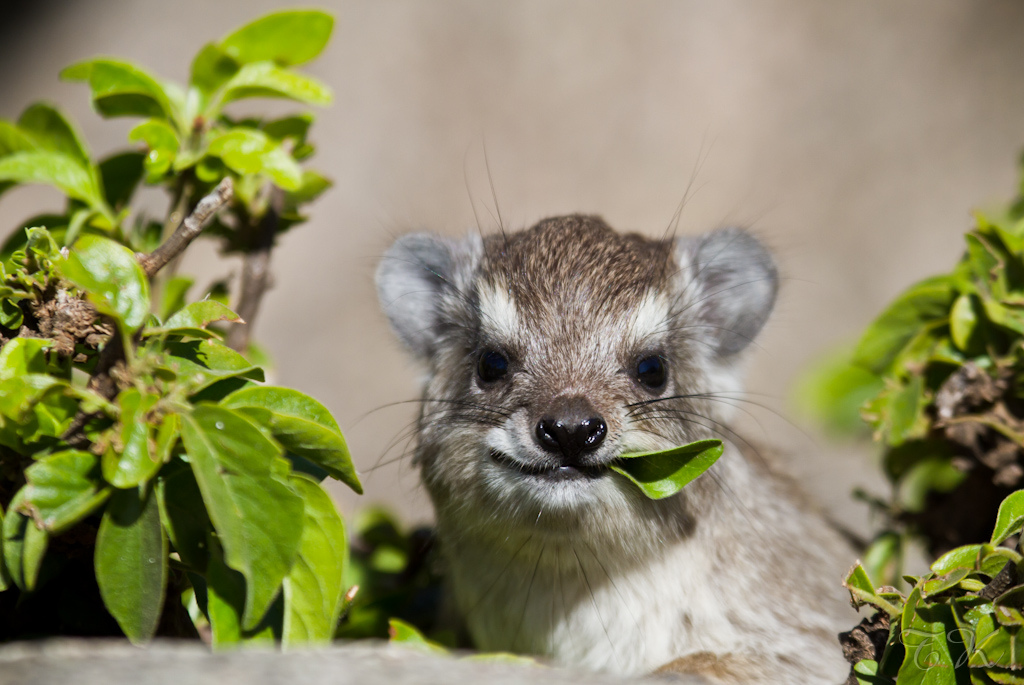
\includegraphics[width=0.4\linewidth]{images/hyraxchew.jpg}\\
  {\tiny Biomathematical Research Centre\\
  University of Canterbury\\
  gvd16@uclive.ac.nz\\
  gvdr.github.io\\}
MMEE - July 9, 2015}


\begin{document}
\frame{\titlepage
\addtocounter{framenumber}{-1}}

\begin{frame}{Why?}

\centering
\begin{tabular}{|c|c|}\hline
Evolution & Ecology \\\hline\hline
Phylogeny & Food Web \\
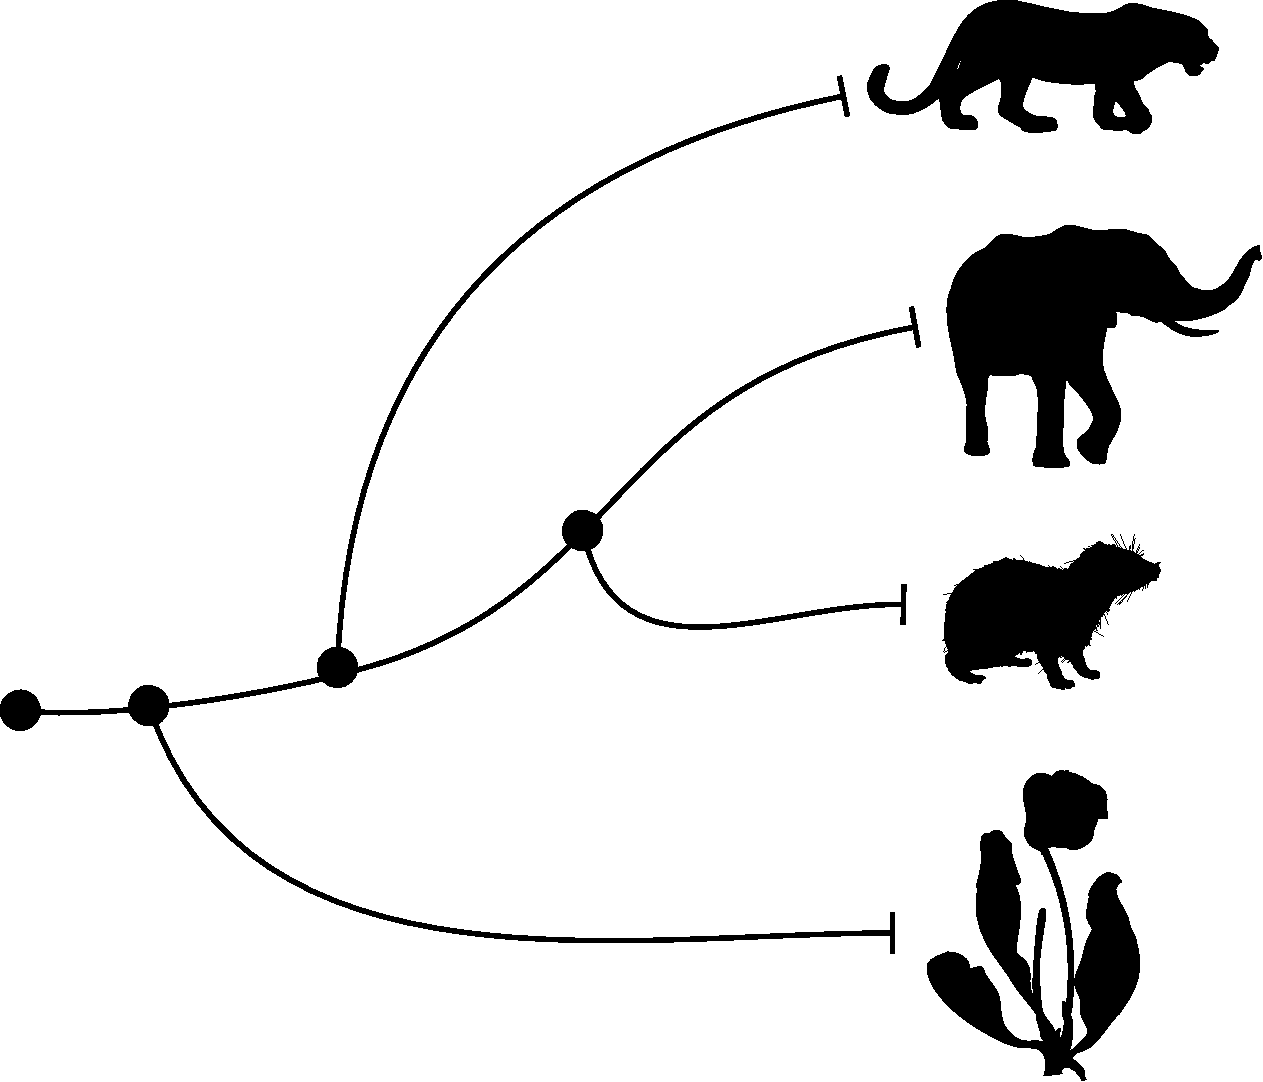
\includegraphics[width=0.4 \textwidth]{images/small_phylo.pdf} & 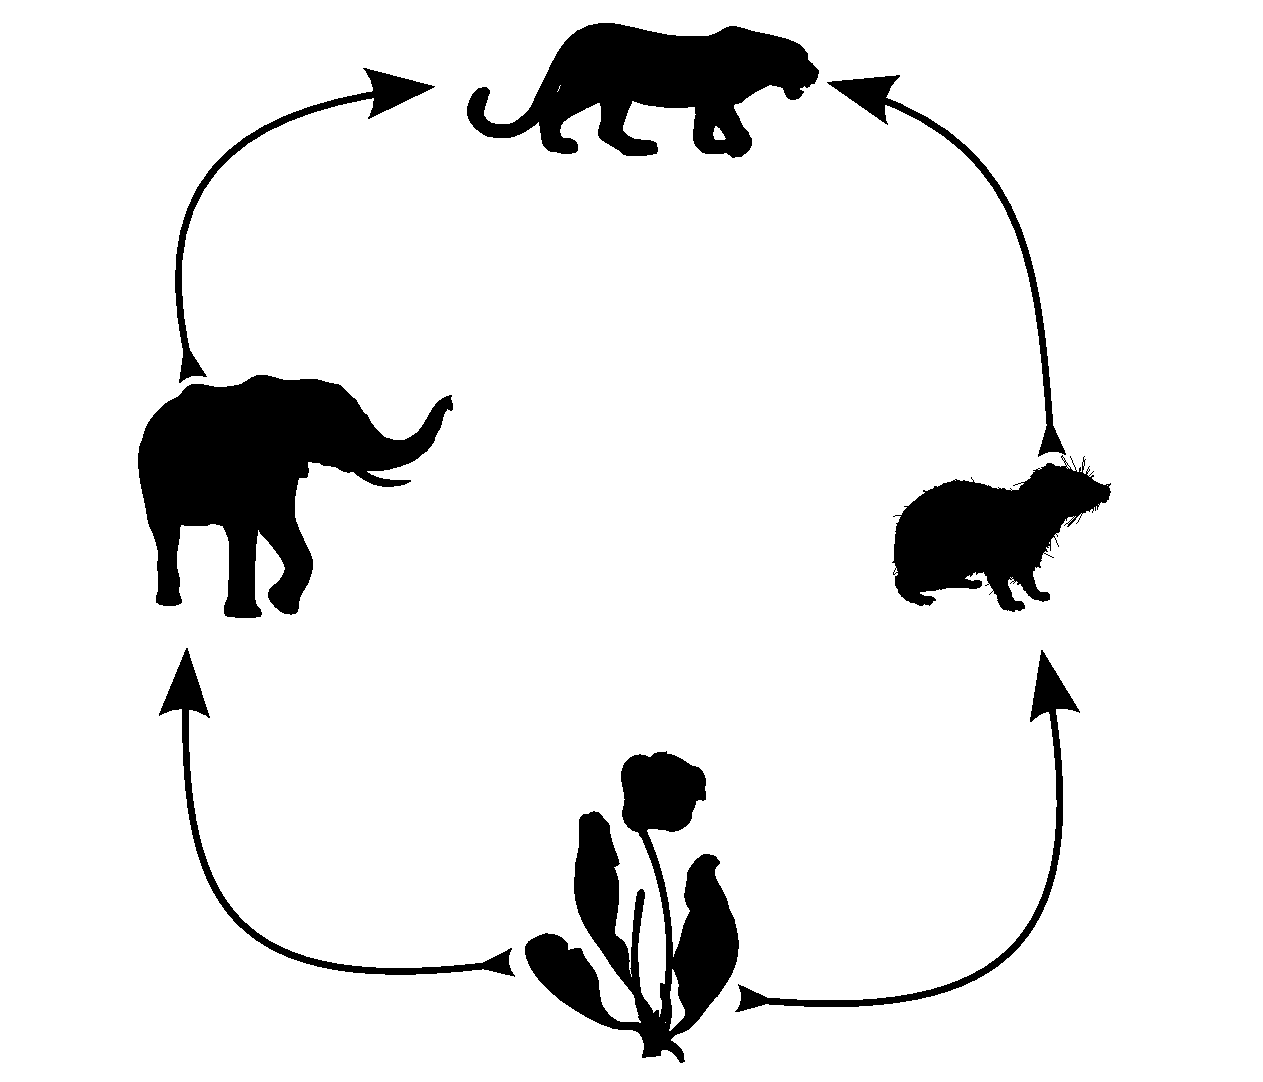
\includegraphics[width=0.4 \textwidth]{images/small_fw.pdf} \\ \hline
\end{tabular}

\tiny{pics from phylopics}
\end{frame}

\begin{frame}{Why?}

\centering
The Theater and the Play

\begin{figure}
\centering
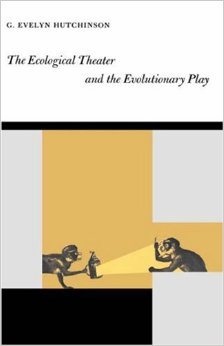
\includegraphics[height=0.5 \textheight]{images/hutchinson_ecotheatreevoplay.jpg}
\end{figure}
\centering
{\tiny Ecology and Evolution occur on different time scales?}

\end{frame}

\begin{frame}{Why?}


\begin{quote}
Although species evolve and diversify in a complex network of species interactions, current models of diversification typically ignore species interactions. Inference approaches basedon joint phylogenetic and species interaction data allow testing the degree to which species interactions are evolutionarily conserved (Ives and Godfray 2006; Rezende et al. 2007), but do not allow analysing the effect of species interactions on diversification.

Helen Morlon - \textit{Ecology Letters} (2014) \textbf{17}: 508-525
\end{quote}

\end{frame}

\begin{frame}{Why?}

\centering
It's hard to fit a Web on a Tree because of all the fine wirings.

\centering
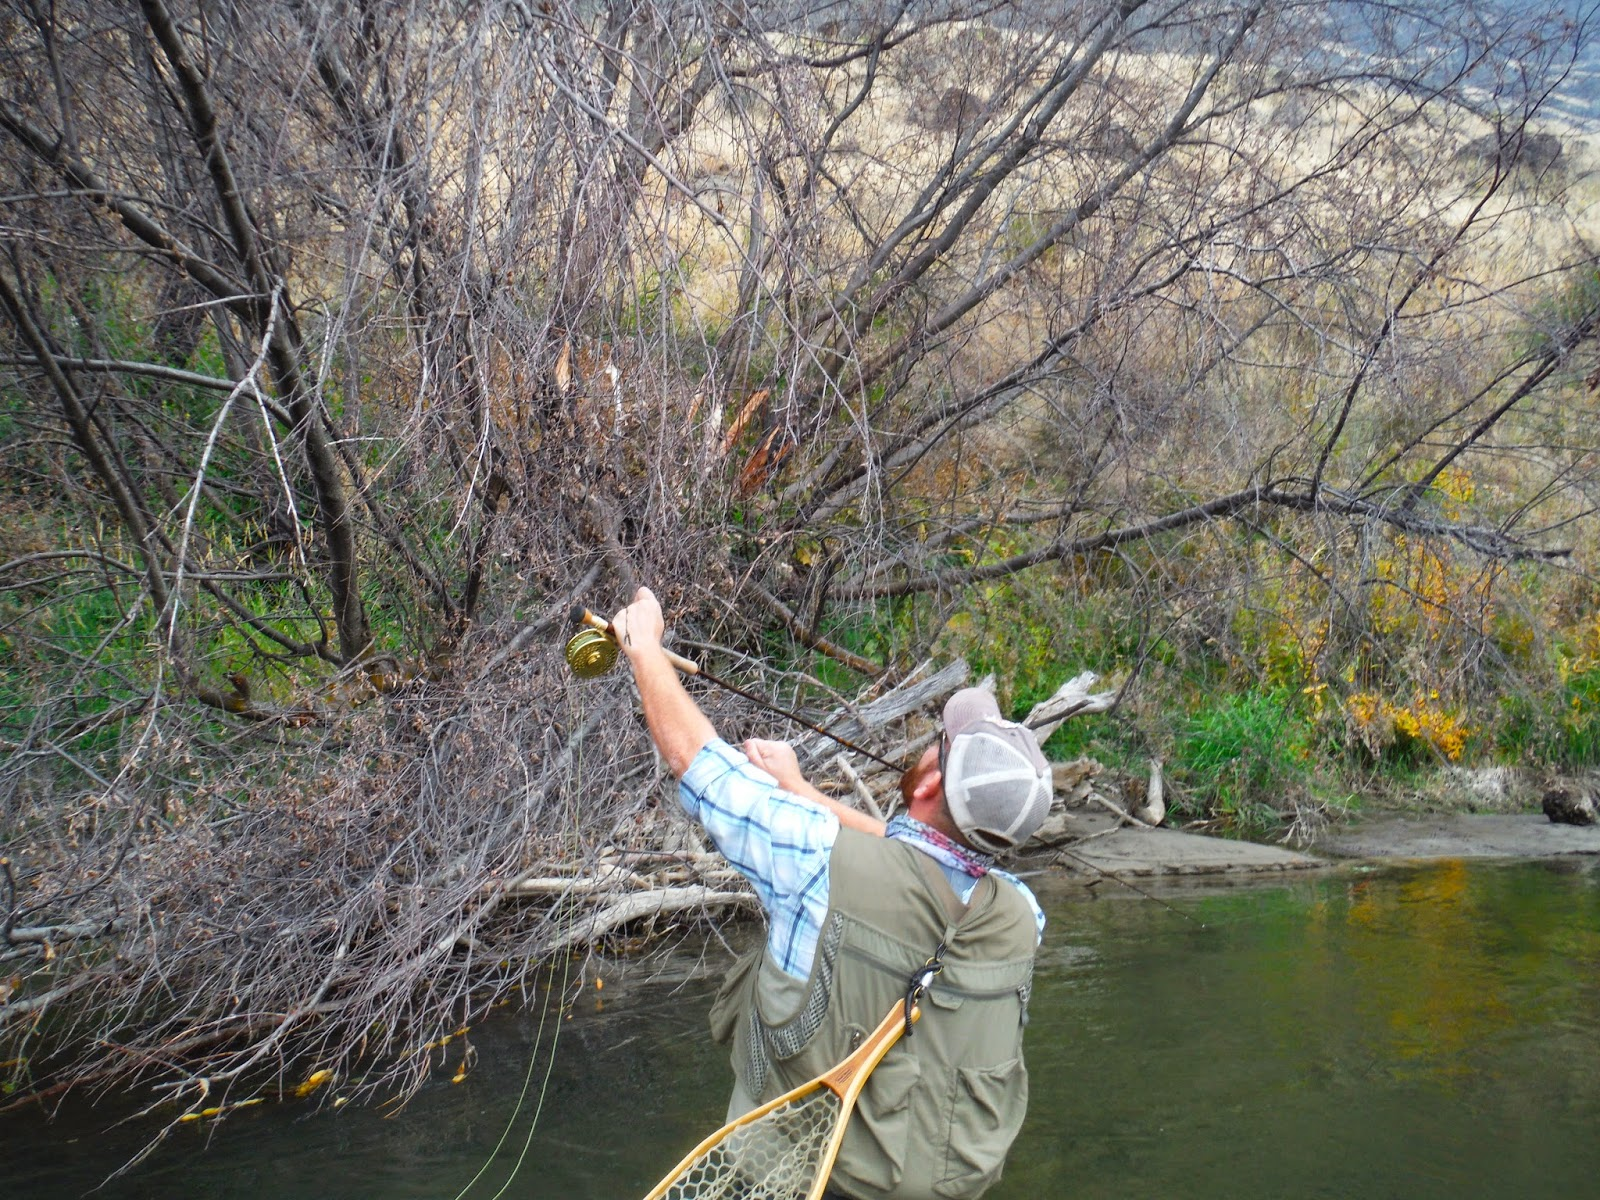
\includegraphics[height=0.5 \textheight]{images/finewirings.jpg}

\centering
{\tiny Courtesy of Erik Moncada}

\end{frame}

\begin{frame}{Why?}

\centering
And you don't always get something out of it.

\centering
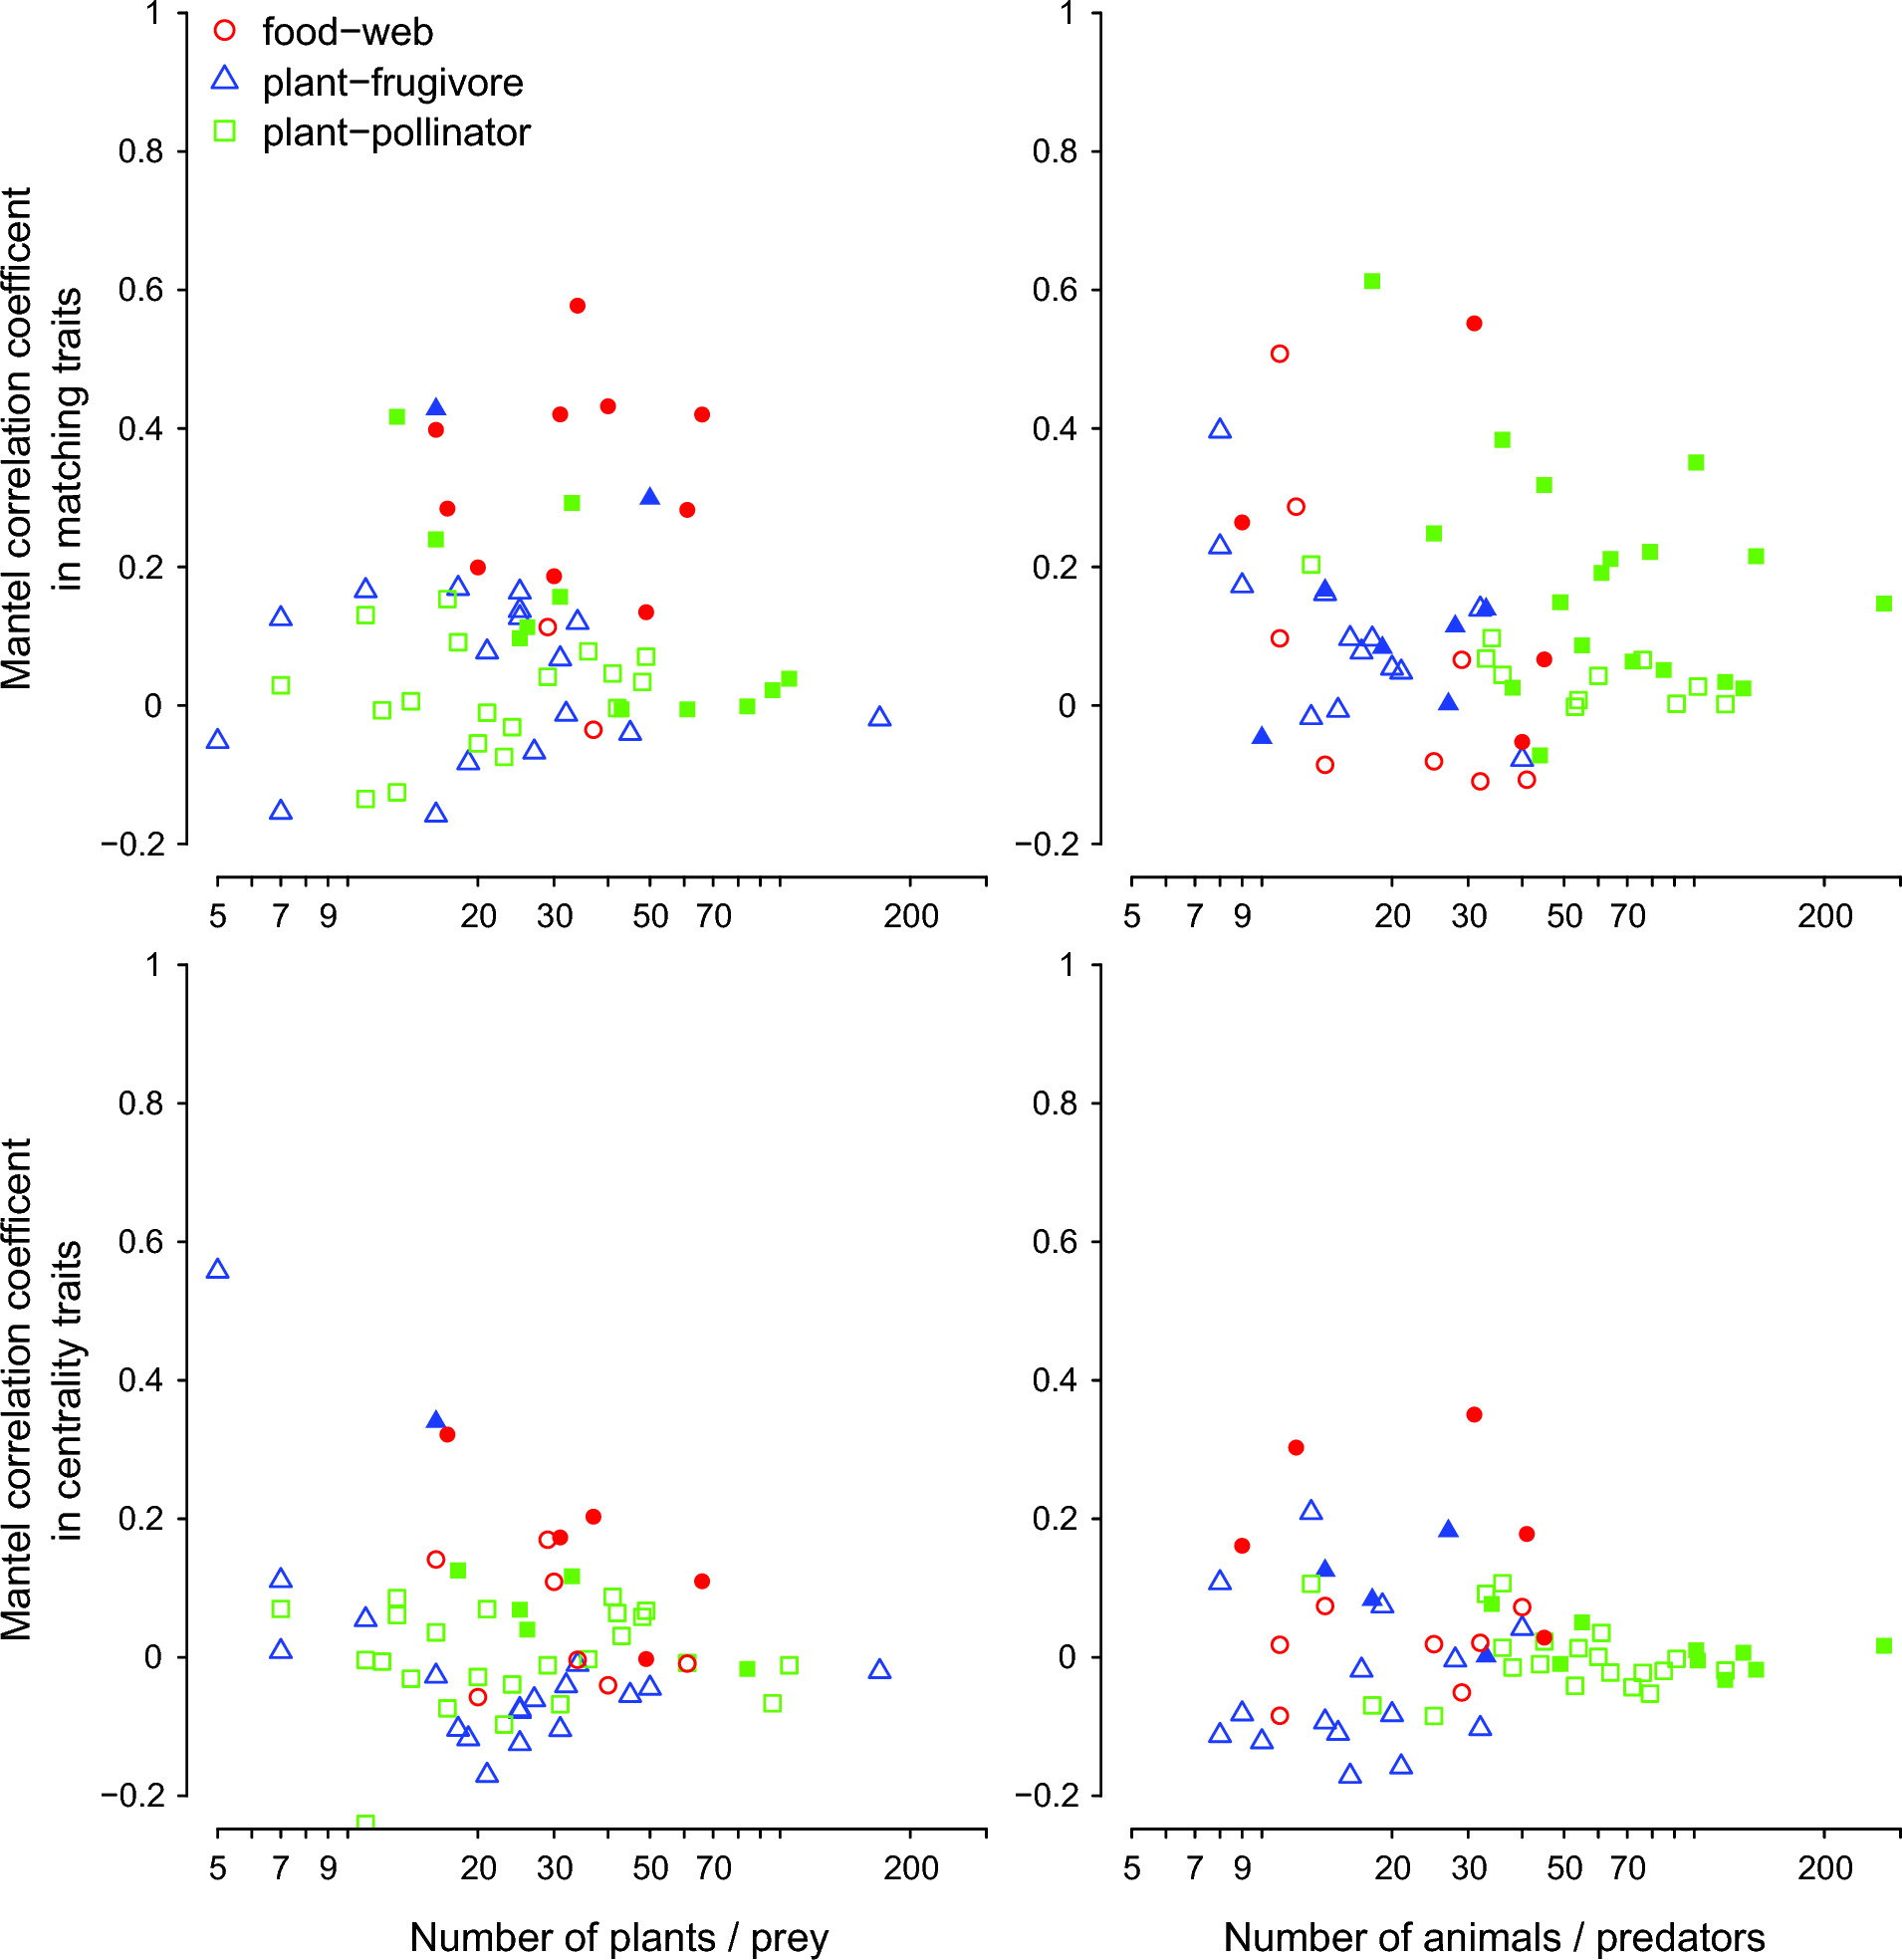
\includegraphics[height=0.7 \textheight]{images/rohr.jpg}

\centering
{\tiny Rohr \& Bascompte, Am Nat 184, 5 (2014)}


\end{frame}


\begin{frame}{What?}

\centering
\begin{tabular}{cc}
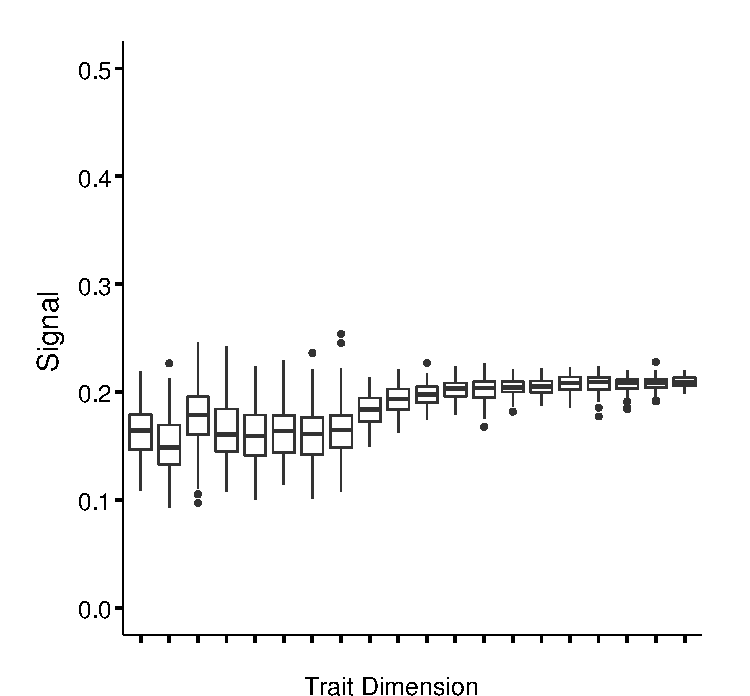
\includegraphics[width=0.47\linewidth]{images/psig.pdf} & 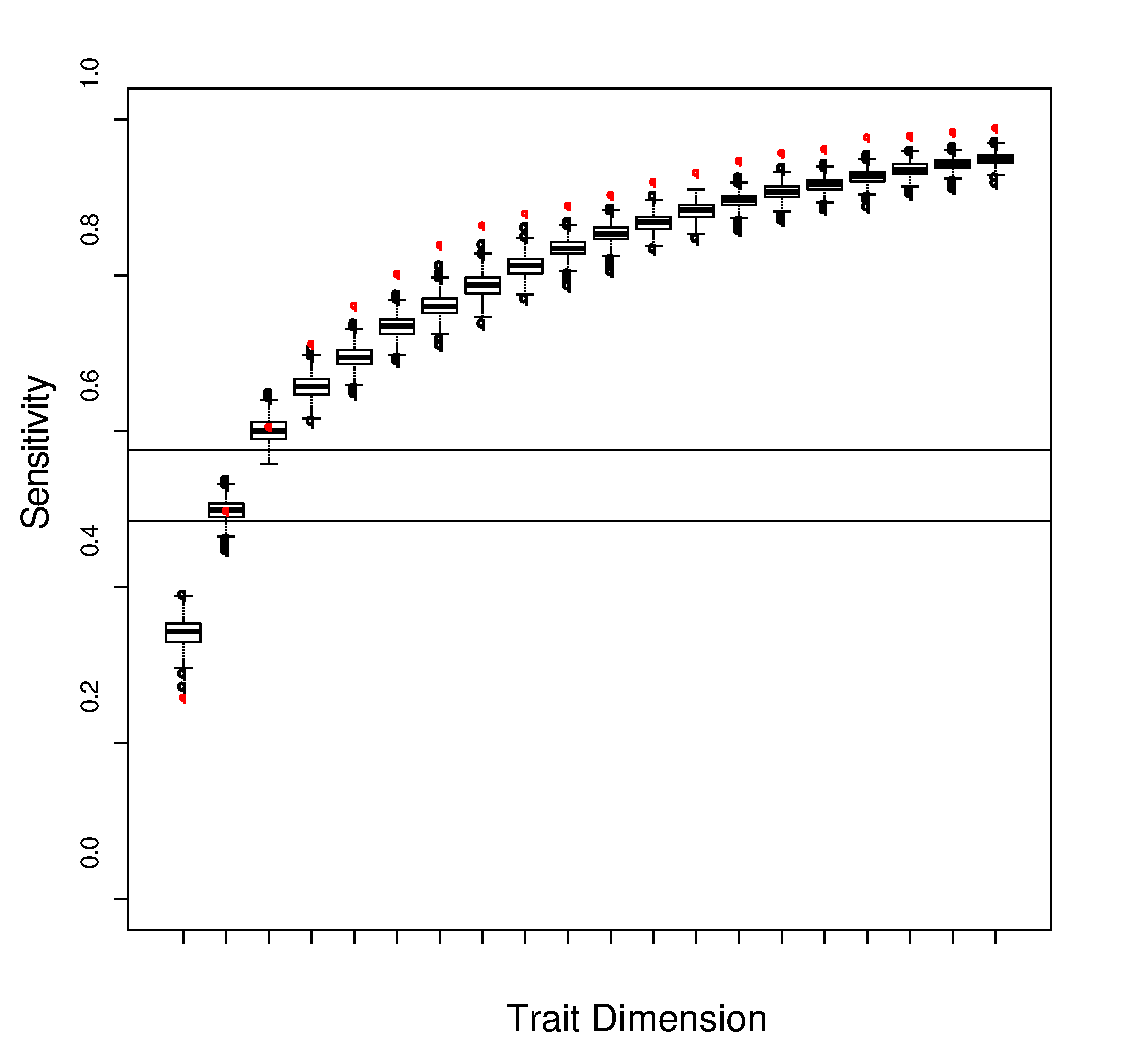
\includegraphics[width=0.47 \linewidth]{images/sens.pdf}\\
{\tiny Phylogenetic signal} & {\tiny Model sensitivity}
\end{tabular}\footnote{From gvdr \& Stouffer, in press}

\centering
The food web's backbones web exhibits Evolutionary signal.

\end{frame}


\begin{frame}{Food Webs embedded}

\centering
\begin{itemize}[<+->]
\itemsep1pt\parskip0pt\parsep0pt
\item
From $G=(V,E)$ to a metric space and back via\\
Random Dot Product Graph
\item
$\mathbb{P}\left( i \to j\right) = \mathbb{T}_{out}\left(i\right) \cdot  \mathbb{T}_{in}\left(j\right)$
\item
SVD(Adjacency) gives $\mathbb{T}_{out}$ and $ \mathbb{T}_{in}$
\end{itemize}

\end{frame}

\begin{frame}{Food Webs embedded}


\centering
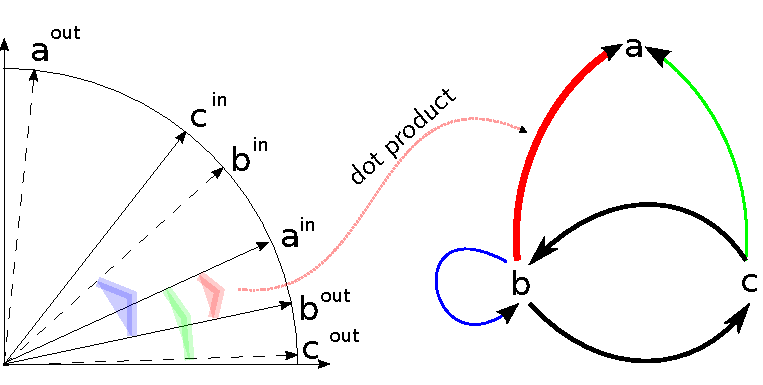
\includegraphics[width=0.9\linewidth]{images/RDPGmodel.pdf}

\end{frame}

\begin{frame}{Food Webs embedded}

\centering
  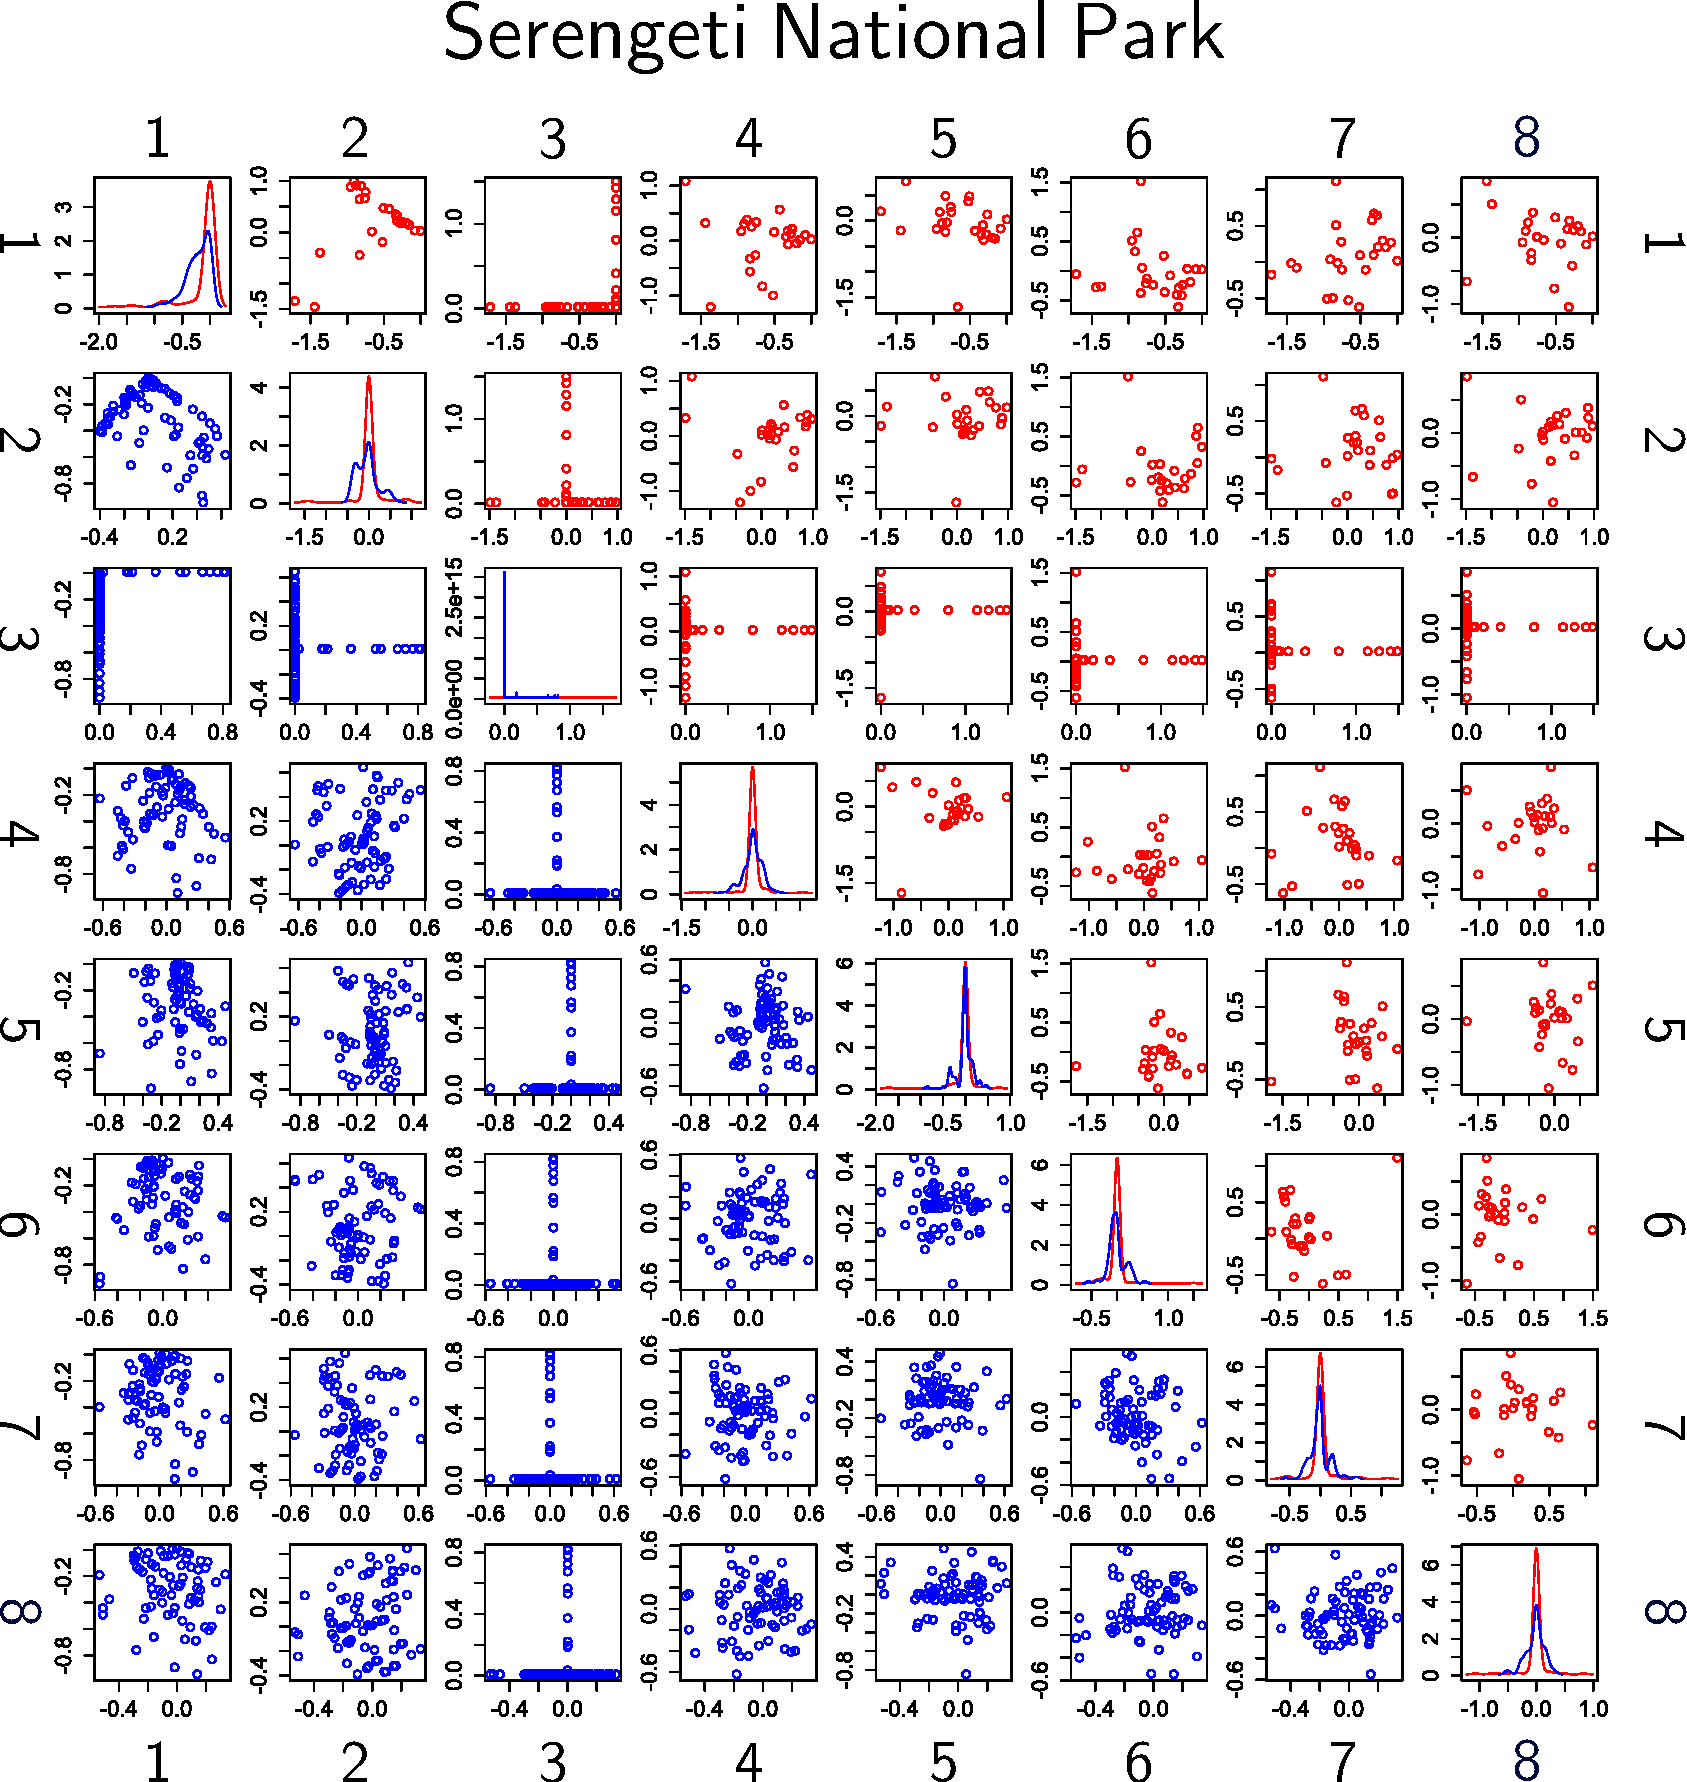
\includegraphics[width=0.6\linewidth]{images/Serengeti_scatter_8.pdf}

\centering
{\tiny A Food Web as you've never seen it. And don't want to see again.}
 
\end{frame}

\begin{frame}{Food Webs embedded}

\centering
  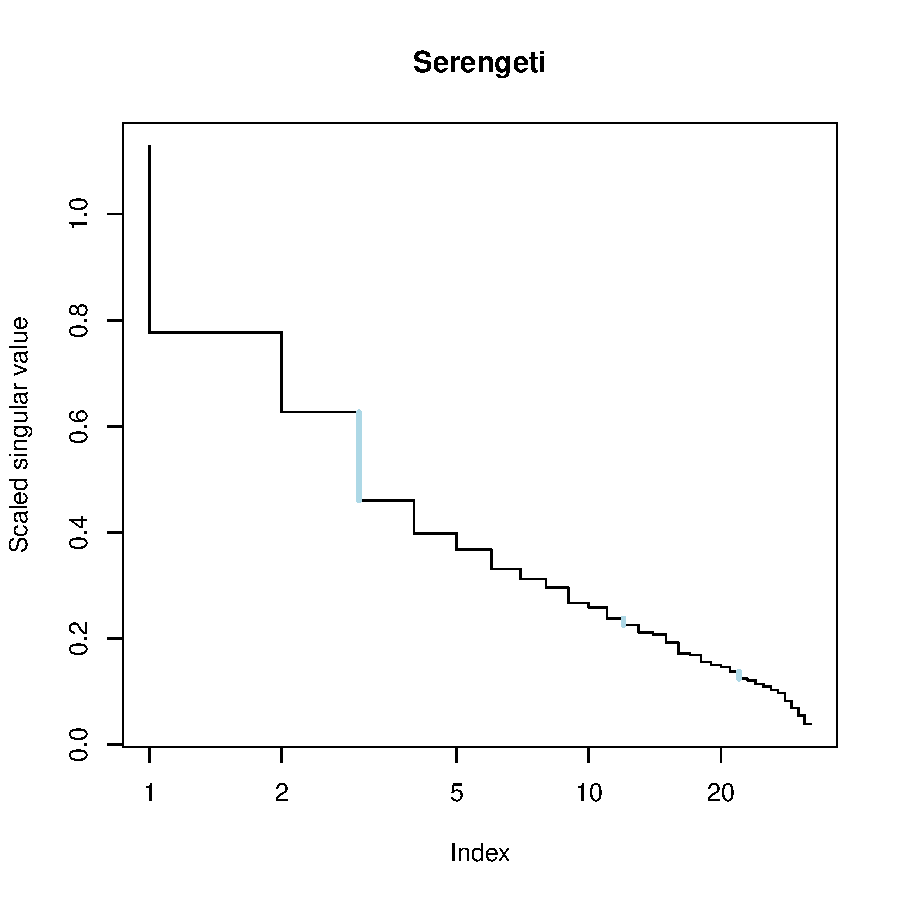
\includegraphics[width=0.4\linewidth]{images/Serengeti_svds.pdf}
  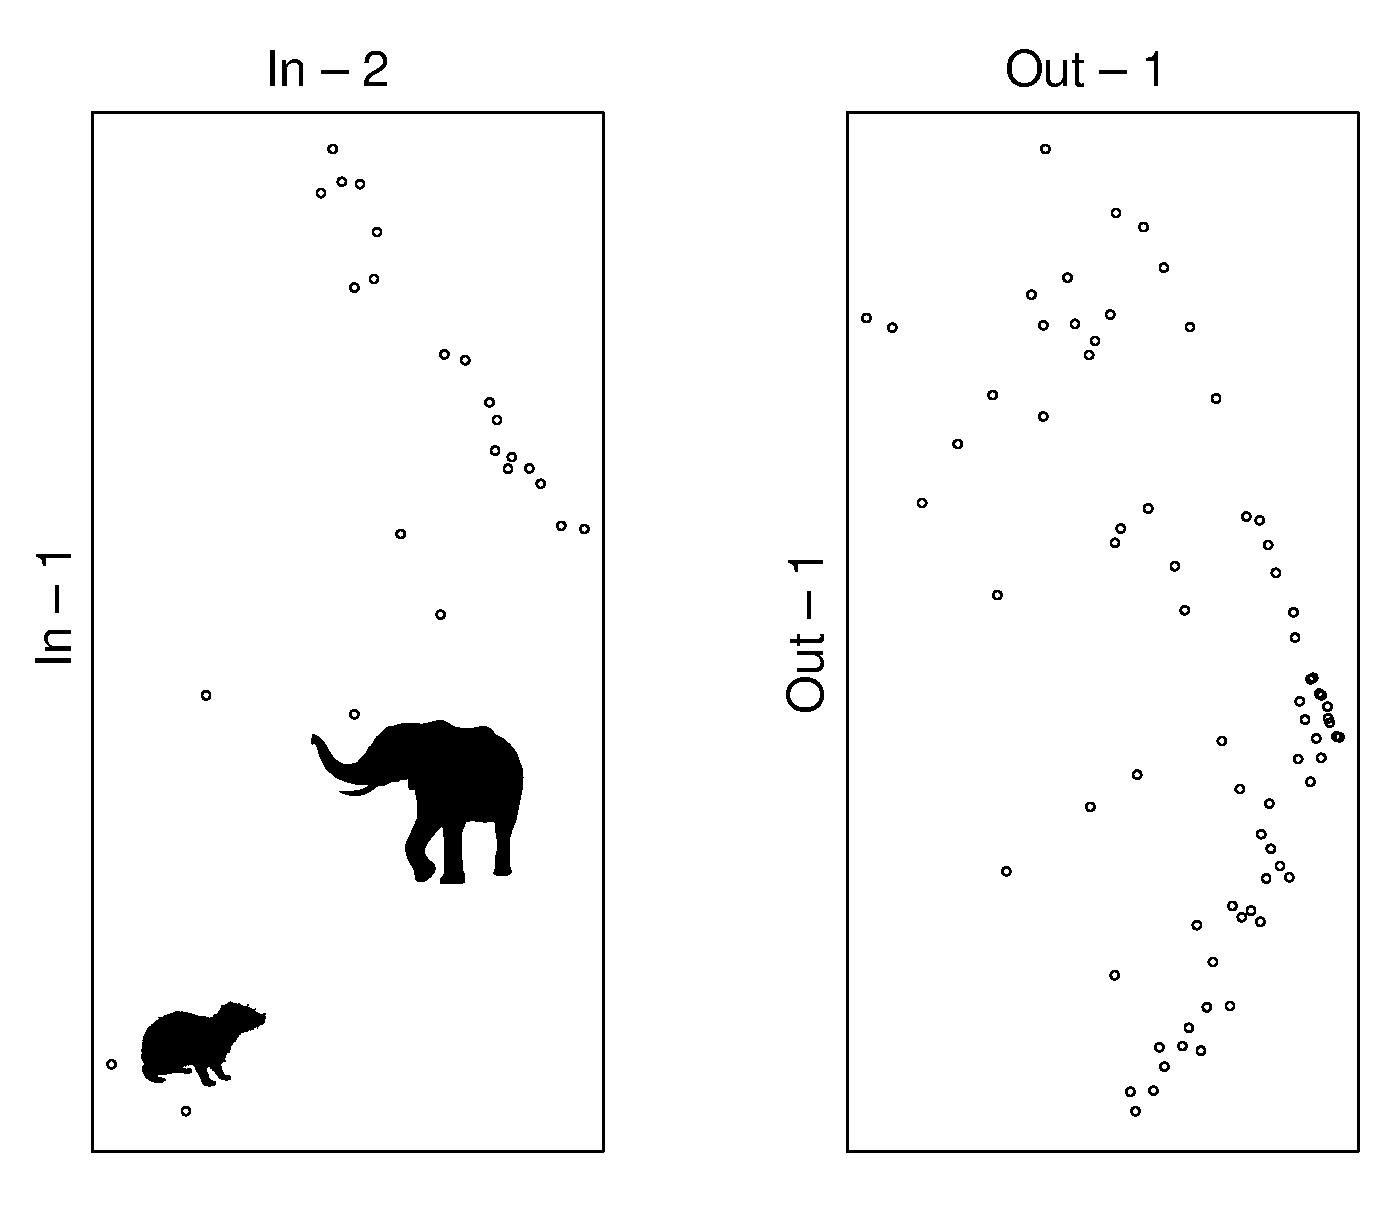
\includegraphics[width=0.6\linewidth]{images/Serengeti_Traits.pdf}

\centering
{\tiny We can choose dimensionality based on singular values.}
 
\end{frame}

\begin{frame}{PCM crash course}

\centering
Expected vs.~Observed trait distribution

  \begin{equation*}
    \textrm{vcv}\left(  \mathbb{T} | \tau, \mbox{null model} \right) \mbox{ vs. } \textrm{vcv}\left( \mathbb{T}\right)
  \end{equation*}

\end{frame}

\begin{frame}{PCM crash course}

\centering

\begin{itemize}[<+->]
\itemsep1pt\parskip0pt\parsep0pt
\item
But what null model?
\item
Brownian Motion:

\begin{equation*}
\mathrm{d} \mathbb{T}(i,t) = \sigma \mathrm{d}B(t)
\end{equation*}
eventually $\sigma = \sigma(i,t)$, e.g., $\sigma(t) = \sigma_0 e^{rt}$.

\item
Ornstein-Uhlenbeck (BM + rubber band):

\begin{equation*}
\mathrm{d} \mathbb{T}(i,t) = \alpha \left( \Theta -  \mathbb{T}(i,t) \right)\mathrm{d}t  + \sigma \mathrm{d}B(t)
\end{equation*}
eventually $\alpha = \alpha(i,t)$ and/or $\Theta = \Theta(i,t)$, ``branch colouring''.

\end{itemize}

\end{frame}

\begin{frame}{More questions (than answers)}

\begin{itemize}[<+->]
\itemsep1pt\parskip0pt\parsep0pt
\item
  There is phylogenetic signal\\
  {\tiny p-values told me...}
\item
  It is quite weak\\
  {\tiny $20\% ~ 30\%$ of variation explained}
\item
  It saturates with dimensionality\\
  {\tiny $d \in \left\{2, \dots , 8 \right\}$}
\item
  $\therefore$ ``fine wirings'' may be deceiving
\item
  Evolutionary model is (a bit) inadequate\\
  {\tiny no interaction effects}
\end{itemize}

\end{frame}

\begin{frame}{(Not a) Conclusion}

\begin{itemize}[<+->]
\item
  Evolutionary distinctiveness vs. Web Centrality\\
  {\small Do evolutionary unique species play a keystone role in Food Webs?}
  \vspace{3 mm}
  
\centering
  
\includegraphics[width=0.4\linewidth]{images/hyraxElephant.pdf}
  
  \vspace{3 mm}

\item
  An ecological informed model of species evolution 
  it's (almost) there.\\
  {\small Consider an Ornstein and Uhlenbeck process and ask:\\
  What if $\Theta = \Theta(i,T(t))$ depends on the traits distribution?}
\end{itemize}

\end{frame}

\begin{frame}{Thanks!}

\begin{centering}
\small{
Joint work with  
Daniel B. Stouffer (University of Canterbury)

Many thanks to  
Mike Steel; Carey Priebe; A. Mooers', D.B. Stouffer's \& J. Tylianakis' labs; ...

Funds by the Allan Wilson Centre for Molecular Ecology and Evolution.}

\centering
  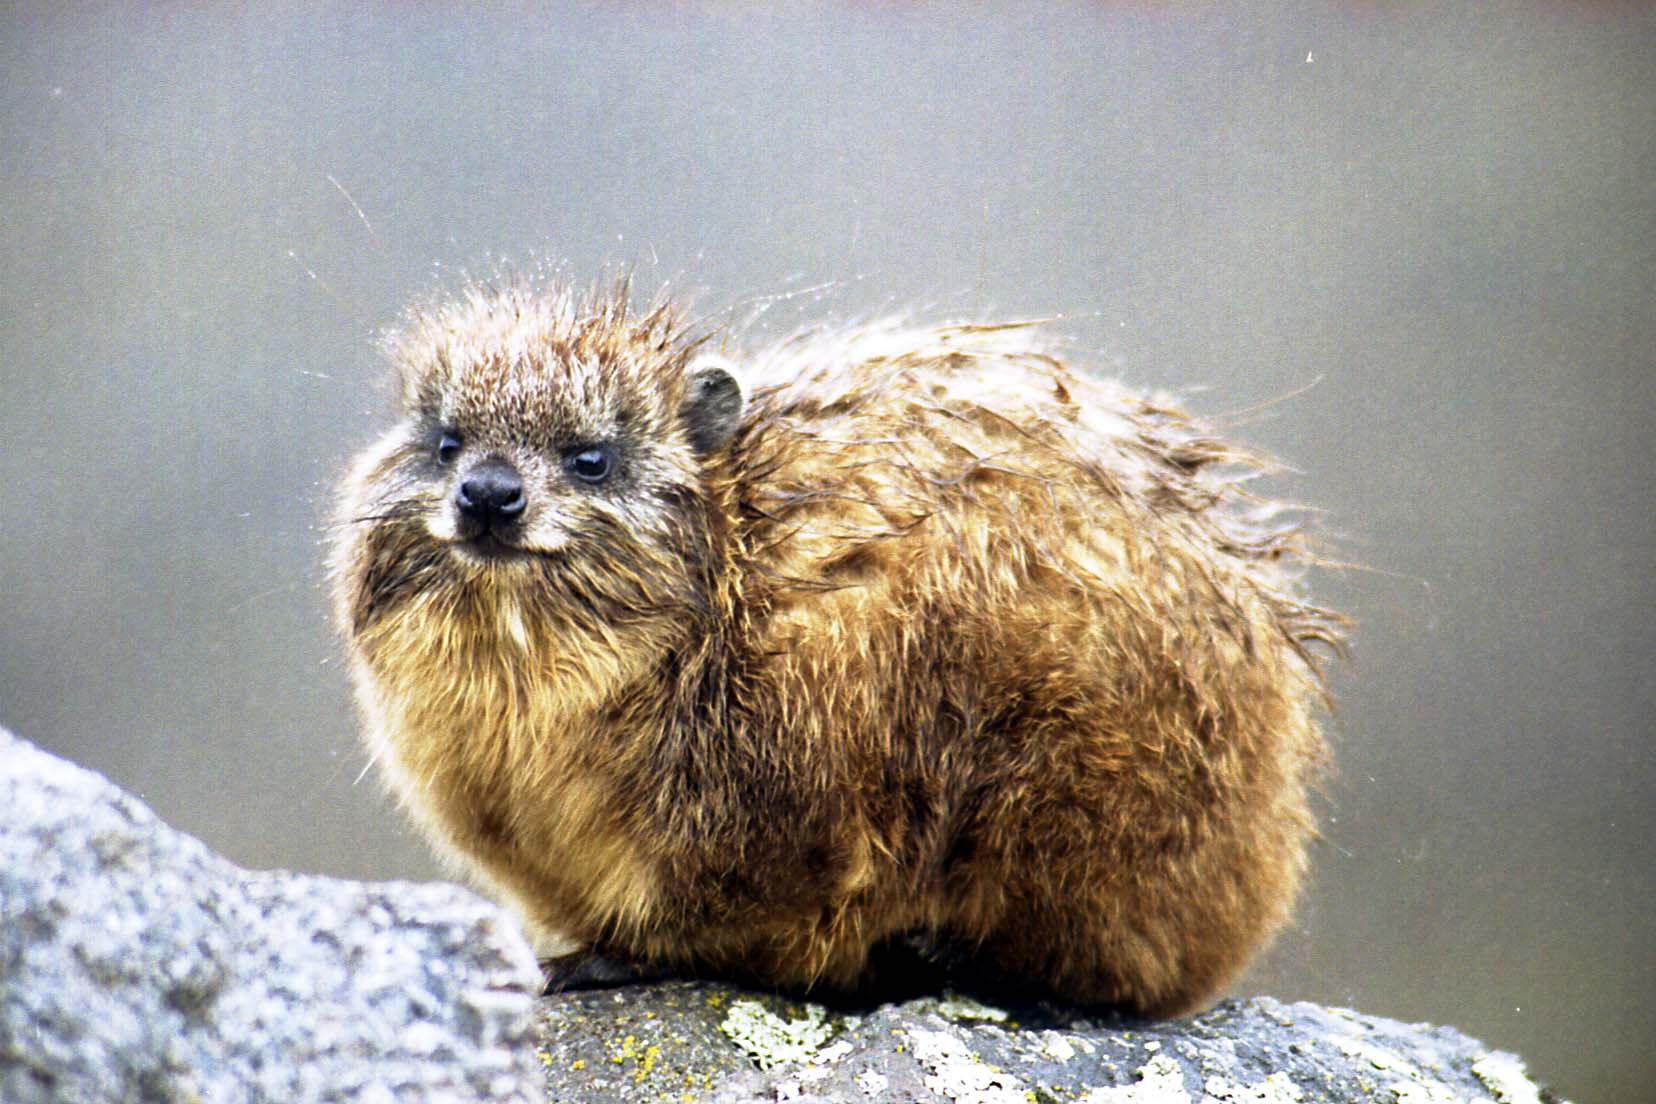
\includegraphics[width=0.4\linewidth]{images/hyrax.jpg}

\small{By the way, I'm currently looking for a postdoc position.\\ gvd16@uclive.ac.nz - gvdr.github.io}

\end{centering}

\end{frame}

\end{document}
